\documentclass{beamer}

%\setbeamersize{text margin left=7.5mm,text margin right=7.5mm}
\usepackage{tikz}

\usepackage{graphicx}
\usepackage[utf8]{inputenc}
\usepackage[T1]{fontenc}
\usepackage[english]{babel}
\usepackage{listings}
\usepackage{xcolor}
\usepackage{eso-pic}
\usepackage{mathrsfs}
\usepackage{url}
\usepackage{amssymb}
\usepackage{amsmath}
\usepackage{multirow}
\usepackage{subcaption}
\usepackage{hyperref}
\usepackage{booktabs}
\usepackage{eurosym}
\usepackage{bm}
\usepackage{cooltooltips}
\usepackage{colordef}
\usepackage{beamerdefs}
\usepackage{lvblisting}


\newcommand{\matr}[1]{\mathbf{#1}} % undergraduate algebra version
%\newcommand{\matr}[1]{#1}          % pure math version
%\newcommand{\matr}[1]{\bm{#1}}     % ISO complying version

% Bibliography
\usepackage[backend=biber,style=authoryear,sorting=nyt]{biblatex}
\usepackage[autostyle,autopunct]{csquotes} % For Quotations
\renewcommand{\mkcitation}[1]{#1} % For correct footcites with csquotes
\addbibresource{references.bib}

\pgfdeclareimage[height=2cm]{logobig}{template/hulogo}
\pgfdeclareimage[height=0.7cm]{logosmall}{images/timeuse.png}


\setbeamercolor{block body alerted}{bg=alerted text.fg!10}
\setbeamercolor{block title alerted}{bg=alerted text.fg!20}
\setbeamercolor{block body}{bg=structure!10}
\setbeamercolor{block title}{bg=structure!20}
\setbeamercolor{block body example}{bg=green!10}
\setbeamercolor{block title example}{bg=green!20}
\setbeamertemplate{blocks}[rounded][shadow]

\renewcommand{\leftcol}{0.6}

\newcommand\myheading[1]{%
  \par\smallskip
  {\large\bfseries#1}\par\smallskip}




% Define Titlepage
\title[Discriminant Analysis for CoDa]{Discriminant Analysis as an Example of Classification Techniques for Compositional Data}

\authora{Manuel Pfeuffer}
\authorb{}
\authorc{}

\def\linka{}
\def\linkb{}
\def\linkc{}

\institute{Seminar: Compositional Data Analysis\\
Humboldt--Universität zu Berlin}

\hypersetup{pdfpagemode=FullScreen}

\begin{document}

% 0-1
%%%%%%%%%%%%%%%%%%%%%%%%%%%%%%%%%%%%%%%%
\frame[plain]{\titlepage}

%%%%%%%%%%%%%%%%%%%%%%%%%%%%%%%%%%%%%%%%
\section{Introduction to Classification and Discriminant Analysis}
%%%%%%%%%%%%%%%%%%%%%%%%%%%%%%%%%%%%%%%%

% 1-1
%%%%%%%%%%%%%%%%%%%%%%%%%%%%%%%%%%%%%%%%
\frame{
\frametitle{When do we need classification techniques?}
\begin{figure}
  \centering
  \input{../output/classification_problem.tex}
\end{figure}
\begin{block}{Classification Problem}
  Given $n$ observations $x_i = (x_{i1}, \dots, x_{ik})$ with \alert{known} class labels $y_i \in \{1,\dots,g\}$, \alert{predict} the class of an unlabelled observation.
\end{block}
}


% 1-2
%%%%%%%%%%%%%%%%%%%%%%%%%%%%%%%%%%%%%%%%
%\frame{
%\frametitle{Simple approach to classification}
%\begin{figure}
%  \centering
%  \input{../output/how_to_classify.tex}
%\end{figure}
%For $j = 1, \dots, g$: 
%\begin{itemize}
%  \item[1.] Calculate class sample mean
%    $\hat{\mu}_j = \frac{1}{n_j} \sum_{i=1}^n I(y_i = j) \cdot x_i$.
%  \item[2.] Calculate distances $\delta_j(x) = \lVert x - \hat{\mu}_j \rVert$
%    from sample means.
%\end{itemize}
%$\Rightarrow$ Classify as class with the smallest distance.
%}


% 1-3
%%%%%%%%%%%%%%%%%%%%%%%%%%%%%%%%%%%%%%%%
\frame{
\frametitle{A simple approach to classification}
\begin{figure}
  \centering
  % Created by tikzDevice version 0.12.3 on 2020-01-28 17:47:35
% !TEX encoding = UTF-8 Unicode
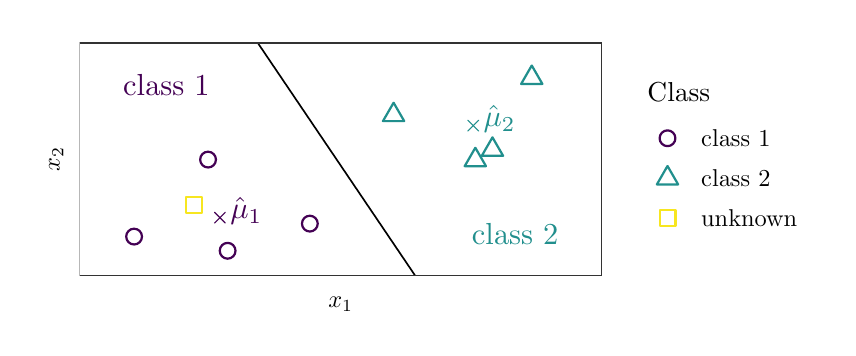
\begin{tikzpicture}[x=1pt,y=1pt]
\definecolor{fillColor}{RGB}{255,255,255}
\path[use as bounding box,fill=fillColor,fill opacity=0.00] (0,0) rectangle (289.08,108.41);
\begin{scope}
\path[clip] (  0.00,  0.00) rectangle (289.08,108.41);
\definecolor{drawColor}{RGB}{255,255,255}
\definecolor{fillColor}{RGB}{255,255,255}

\path[draw=drawColor,line width= 0.6pt,line join=round,line cap=round,fill=fillColor] (  0.00,  0.00) rectangle (289.08,108.41);
\end{scope}
\begin{scope}
\path[clip] ( 18.77, 18.77) rectangle (207.47,102.91);
\definecolor{fillColor}{RGB}{255,255,255}

\path[fill=fillColor] ( 18.77, 18.77) rectangle (207.47,102.91);
\definecolor{drawColor}{RGB}{68,1,84}

\path[draw=drawColor,line width= 0.8pt,line join=round,line cap=round] ( 72.25, 27.79) circle (  2.85);

\path[draw=drawColor,line width= 0.8pt,line join=round,line cap=round] ( 38.45, 32.92) circle (  2.85);

\path[draw=drawColor,line width= 0.8pt,line join=round,line cap=round] ( 65.18, 60.74) circle (  2.85);

\path[draw=drawColor,line width= 0.8pt,line join=round,line cap=round] (101.96, 37.60) circle (  2.85);
\definecolor{drawColor}{RGB}{33,143,141}

\path[draw=drawColor,line width= 0.8pt,line join=round,line cap=round] (161.76, 65.03) --
	(165.61, 58.37) --
	(157.92, 58.37) --
	(161.76, 65.03);

\path[draw=drawColor,line width= 0.8pt,line join=round,line cap=round] (167.95, 68.78) --
	(171.79, 62.12) --
	(164.10, 62.12) --
	(167.95, 68.78);

\path[draw=drawColor,line width= 0.8pt,line join=round,line cap=round] (182.15, 94.74) --
	(185.99, 88.08) --
	(178.31, 88.08) --
	(182.15, 94.74);

\path[draw=drawColor,line width= 0.8pt,line join=round,line cap=round] (132.22, 81.30) --
	(136.07, 74.64) --
	(128.38, 74.64) --
	(132.22, 81.30);
\definecolor{drawColor}{RGB}{247,230,32}

\path[draw=drawColor,line width= 0.8pt,line join=round,line cap=round] ( 57.20, 41.39) rectangle ( 62.91, 47.10);
\definecolor{drawColor}{RGB}{68,1,84}

\path[draw=drawColor,line width= 0.4pt,line join=round,line cap=round] ( 67.50, 37.80) -- ( 71.42, 41.72);

\path[draw=drawColor,line width= 0.4pt,line join=round,line cap=round] ( 67.50, 41.72) -- ( 71.42, 37.80);
\definecolor{drawColor}{RGB}{33,143,141}

\path[draw=drawColor,line width= 0.4pt,line join=round,line cap=round] (159.06, 71.06) -- (162.98, 74.98);

\path[draw=drawColor,line width= 0.4pt,line join=round,line cap=round] (159.06, 74.98) -- (162.98, 71.06);
\definecolor{drawColor}{RGB}{68,1,84}

\node[text=drawColor,anchor=base,inner sep=0pt, outer sep=0pt, scale=  1.10] at ( 78.99, 39.44) {$\hat{\mu}_1$};
\definecolor{drawColor}{RGB}{33,143,141}

\node[text=drawColor,anchor=base,inner sep=0pt, outer sep=0pt, scale=  1.10] at (170.55, 72.70) {$\hat{\mu}_2$};
\definecolor{drawColor}{RGB}{0,0,0}

\path[draw=drawColor,line width= 0.6pt,line join=round] ( 79.43,108.41) --
	(152.74,  0.00);
\definecolor{drawColor}{RGB}{68,1,84}

\node[text=drawColor,anchor=base west,inner sep=0pt, outer sep=0pt, scale=  1.10] at ( 34.47, 83.90) {class 1};
\definecolor{drawColor}{RGB}{33,143,141}

\node[text=drawColor,anchor=base east,inner sep=0pt, outer sep=0pt, scale=  1.10] at (191.78, 30.18) {class 2};
\definecolor{drawColor}{gray}{0.20}

\path[draw=drawColor,line width= 0.6pt,line join=round,line cap=round] ( 18.77, 18.77) rectangle (207.47,102.91);
\end{scope}
\begin{scope}
\path[clip] (  0.00,  0.00) rectangle (289.08,108.41);
\definecolor{drawColor}{RGB}{0,0,0}

\node[text=drawColor,anchor=base,inner sep=0pt, outer sep=0pt, scale=  0.88] at (113.12,  7.21) {$x_1$};
\end{scope}
\begin{scope}
\path[clip] (  0.00,  0.00) rectangle (289.08,108.41);
\definecolor{drawColor}{RGB}{0,0,0}

\node[text=drawColor,rotate= 90.00,anchor=base,inner sep=0pt, outer sep=0pt, scale=  0.88] at ( 11.56, 60.84) {$x_2$};
\end{scope}
\begin{scope}
\path[clip] (  0.00,  0.00) rectangle (289.08,108.41);
\definecolor{fillColor}{RGB}{255,255,255}

\path[fill=fillColor] (218.47, 26.81) rectangle (283.58, 94.87);
\end{scope}
\begin{scope}
\path[clip] (  0.00,  0.00) rectangle (289.08,108.41);
\definecolor{drawColor}{RGB}{0,0,0}

\node[text=drawColor,anchor=base west,inner sep=0pt, outer sep=0pt, scale=  0.99] at (223.97, 81.59) {Class};
\end{scope}
\begin{scope}
\path[clip] (  0.00,  0.00) rectangle (289.08,108.41);
\definecolor{fillColor}{RGB}{255,255,255}

\path[fill=fillColor] (223.97, 61.22) rectangle (238.43, 75.67);
\end{scope}
\begin{scope}
\path[clip] (  0.00,  0.00) rectangle (289.08,108.41);
\definecolor{drawColor}{RGB}{68,1,84}

\path[draw=drawColor,line width= 0.8pt,line join=round,line cap=round] (231.20, 68.45) circle (  2.85);
\end{scope}
\begin{scope}
\path[clip] (  0.00,  0.00) rectangle (289.08,108.41);
\definecolor{fillColor}{RGB}{255,255,255}

\path[fill=fillColor] (223.97, 46.76) rectangle (238.43, 61.22);
\end{scope}
\begin{scope}
\path[clip] (  0.00,  0.00) rectangle (289.08,108.41);
\definecolor{drawColor}{RGB}{33,143,141}

\path[draw=drawColor,line width= 0.8pt,line join=round,line cap=round] (231.20, 58.43) --
	(235.04, 51.77) --
	(227.36, 51.77) --
	(231.20, 58.43);
\end{scope}
\begin{scope}
\path[clip] (  0.00,  0.00) rectangle (289.08,108.41);
\definecolor{fillColor}{RGB}{255,255,255}

\path[fill=fillColor] (223.97, 32.31) rectangle (238.43, 46.76);
\end{scope}
\begin{scope}
\path[clip] (  0.00,  0.00) rectangle (289.08,108.41);
\definecolor{drawColor}{RGB}{247,230,32}

\path[draw=drawColor,line width= 0.8pt,line join=round,line cap=round] (228.35, 36.68) rectangle (234.05, 42.39);
\end{scope}
\begin{scope}
\path[clip] (  0.00,  0.00) rectangle (289.08,108.41);
\definecolor{drawColor}{RGB}{0,0,0}

\node[text=drawColor,anchor=base west,inner sep=0pt, outer sep=0pt, scale=  0.88] at (243.38, 65.42) {class 1};
\end{scope}
\begin{scope}
\path[clip] (  0.00,  0.00) rectangle (289.08,108.41);
\definecolor{drawColor}{RGB}{0,0,0}

\node[text=drawColor,anchor=base west,inner sep=0pt, outer sep=0pt, scale=  0.88] at (243.38, 50.96) {class 2};
\end{scope}
\begin{scope}
\path[clip] (  0.00,  0.00) rectangle (289.08,108.41);
\definecolor{drawColor}{RGB}{0,0,0}

\node[text=drawColor,anchor=base west,inner sep=0pt, outer sep=0pt, scale=  0.88] at (243.38, 36.51) {unknown};
\end{scope}
\end{tikzpicture}

\end{figure}
\begin{block}{Discriminant Function and Classifier}
  $$ \delta_j(x) = \lVert x - \hat{\mu}_j \rVert, \qquad D(x) =
  \begin{cases}
    \text{"class 1"},& \text{if } 
      \delta_1 < \delta_2 \\
    \text{"class 2"},& \text{otherwise}
  \end{cases}
  $$
\end{block}
}


% 1-4
%%%%%%%%%%%%%%%%%%%%%%%%%%%%%%%%%%%%%%%%
\frame{
\frametitle{A simple approach to classification}
\begin{figure}
\centering
% Created by tikzDevice version 0.12.3 on 2020-01-28 17:47:39
% !TEX encoding = UTF-8 Unicode
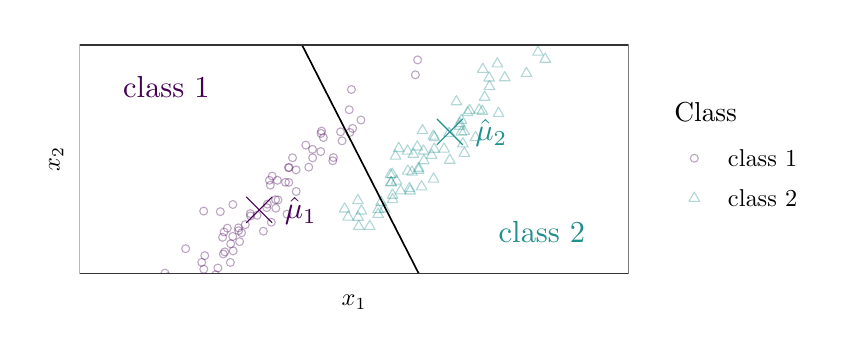
\begin{tikzpicture}[x=1pt,y=1pt]
\definecolor{fillColor}{RGB}{255,255,255}
\path[use as bounding box,fill=fillColor,fill opacity=0.00] (0,0) rectangle (289.08,108.41);
\begin{scope}
\path[clip] (  0.00,  0.74) rectangle (289.08,107.67);
\definecolor{drawColor}{RGB}{255,255,255}
\definecolor{fillColor}{RGB}{255,255,255}

\path[draw=drawColor,line width= 0.6pt,line join=round,line cap=round,fill=fillColor] (  0.00,  0.74) rectangle (289.08,107.67);
\end{scope}
\begin{scope}
\path[clip] ( 18.77, 19.51) rectangle (217.15,102.17);
\definecolor{fillColor}{RGB}{255,255,255}

\path[fill=fillColor] ( 18.77, 19.51) rectangle (217.15,102.17);
\definecolor{drawColor}{RGB}{68,1,84}

\path[draw=drawColor,draw opacity=0.35,line width= 0.4pt,line join=round,line cap=round] ( 55.91, 11.00) circle (  1.43);

\path[draw=drawColor,draw opacity=0.35,line width= 0.4pt,line join=round,line cap=round] ( 69.60, 41.92) circle (  1.43);

\path[draw=drawColor,draw opacity=0.35,line width= 0.4pt,line join=round,line cap=round] ( 50.55, 18.40) circle (  1.43);

\path[draw=drawColor,draw opacity=0.35,line width= 0.4pt,line join=round,line cap=round] ( 63.63, 21.13) circle (  1.43);

\path[draw=drawColor,draw opacity=0.35,line width= 0.4pt,line join=round,line cap=round] ( 68.73, 21.57) circle (  1.43);

\path[draw=drawColor,draw opacity=0.35,line width= 0.4pt,line join=round,line cap=round] (102.92, 64.45) circle (  1.43);

\path[draw=drawColor,draw opacity=0.35,line width= 0.4pt,line join=round,line cap=round] ( 86.63, 44.67) circle (  1.43);

\path[draw=drawColor,draw opacity=0.35,line width= 0.4pt,line join=round,line cap=round] ( 53.32,  9.86) circle (  1.43);

\path[draw=drawColor,draw opacity=0.35,line width= 0.4pt,line join=round,line cap=round] (117.41, 72.00) circle (  1.43);

\path[draw=drawColor,draw opacity=0.35,line width= 0.4pt,line join=round,line cap=round] ( 93.13, 52.56) circle (  1.43);

\path[draw=drawColor,draw opacity=0.35,line width= 0.4pt,line join=round,line cap=round] ( 76.59, 31.10) circle (  1.43);

\path[draw=drawColor,draw opacity=0.35,line width= 0.4pt,line join=round,line cap=round] (110.24, 60.31) circle (  1.43);

\path[draw=drawColor,draw opacity=0.35,line width= 0.4pt,line join=round,line cap=round] (105.90, 63.65) circle (  1.43);

\path[draw=drawColor,draw opacity=0.35,line width= 0.4pt,line join=round,line cap=round] (100.50, 65.96) circle (  1.43);

\path[draw=drawColor,draw opacity=0.35,line width= 0.4pt,line join=round,line cap=round] (101.56, 58.01) circle (  1.43);

\path[draw=drawColor,draw opacity=0.35,line width= 0.4pt,line join=round,line cap=round] ( 94.47, 57.89) circle (  1.43);

\path[draw=drawColor,draw opacity=0.35,line width= 0.4pt,line join=round,line cap=round] ( 85.17, 34.88) circle (  1.43);

\path[draw=drawColor,draw opacity=0.35,line width= 0.4pt,line join=round,line cap=round] ( 74.10, 32.96) circle (  1.43);

\path[draw=drawColor,draw opacity=0.35,line width= 0.4pt,line join=round,line cap=round] ( 70.42, 32.66) circle (  1.43);

\path[draw=drawColor,draw opacity=0.35,line width= 0.4pt,line join=round,line cap=round] ( 62.90, 23.62) circle (  1.43);

\path[draw=drawColor,draw opacity=0.35,line width= 0.4pt,line join=round,line cap=round] ( 76.16, 36.06) circle (  1.43);

\path[draw=drawColor,draw opacity=0.35,line width= 0.4pt,line join=round,line cap=round] ( 50.89,  5.60) circle (  1.43);

\path[draw=drawColor,draw opacity=0.35,line width= 0.4pt,line join=round,line cap=round] (140.92, 96.76) circle (  1.43);

\path[draw=drawColor,draw opacity=0.35,line width= 0.4pt,line join=round,line cap=round] (116.43, 70.56) circle (  1.43);

\path[draw=drawColor,draw opacity=0.35,line width= 0.4pt,line join=round,line cap=round] ( 52.30, 11.64) circle (  1.43);

\path[draw=drawColor,draw opacity=0.35,line width= 0.4pt,line join=round,line cap=round] ( 74.27, 27.74) circle (  1.43);

\path[draw=drawColor,draw opacity=0.35,line width= 0.4pt,line join=round,line cap=round] ( 71.23, 27.39) circle (  1.43);

\path[draw=drawColor,draw opacity=0.35,line width= 0.4pt,line join=round,line cap=round] (102.97, 61.39) circle (  1.43);

\path[draw=drawColor,draw opacity=0.35,line width= 0.4pt,line join=round,line cap=round] ( 74.14, 44.51) circle (  1.43);

\path[draw=drawColor,draw opacity=0.35,line width= 0.4pt,line join=round,line cap=round] ( 90.46, 46.15) circle (  1.43);

\path[draw=drawColor,draw opacity=0.35,line width= 0.4pt,line join=round,line cap=round] ( 80.44, 41.23) circle (  1.43);

\path[draw=drawColor,draw opacity=0.35,line width= 0.4pt,line join=round,line cap=round] ( 80.54, 40.38) circle (  1.43);

\path[draw=drawColor,draw opacity=0.35,line width= 0.4pt,line join=round,line cap=round] (120.42, 75.04) circle (  1.43);

\path[draw=drawColor,draw opacity=0.35,line width= 0.4pt,line join=round,line cap=round] ( 76.23, 35.06) circle (  1.43);

\path[draw=drawColor,draw opacity=0.35,line width= 0.4pt,line join=round,line cap=round] (116.99, 86.08) circle (  1.43);

\path[draw=drawColor,draw opacity=0.35,line width= 0.4pt,line join=round,line cap=round] ( 40.21,  1.24) circle (  1.43);

\path[draw=drawColor,draw opacity=0.35,line width= 0.4pt,line join=round,line cap=round] ( 96.98, 57.04) circle (  1.43);

\path[draw=drawColor,draw opacity=0.35,line width= 0.4pt,line join=round,line cap=round] ( 86.39, 43.37) circle (  1.43);

\path[draw=drawColor,draw opacity=0.35,line width= 0.4pt,line join=round,line cap=round] ( 93.72, 41.02) circle (  1.43);

\path[draw=drawColor,draw opacity=0.35,line width= 0.4pt,line join=round,line cap=round] ( 88.35, 54.78) circle (  1.43);

\path[draw=drawColor,draw opacity=0.35,line width= 0.4pt,line join=round,line cap=round] ( 73.24, 23.57) circle (  1.43);

\path[draw=drawColor,draw opacity=0.35,line width= 0.4pt,line join=round,line cap=round] ( 70.98, 34.58) circle (  1.43);

\path[draw=drawColor,draw opacity=0.35,line width= 0.4pt,line join=round,line cap=round] ( 49.61, 19.71) circle (  1.43);

\path[draw=drawColor,draw opacity=0.35,line width= 0.4pt,line join=round,line cap=round] ( 58.36,  8.41) circle (  1.43);

\path[draw=drawColor,draw opacity=0.35,line width= 0.4pt,line join=round,line cap=round] ( 87.67, 51.48) circle (  1.43);

\path[draw=drawColor,draw opacity=0.35,line width= 0.4pt,line join=round,line cap=round] ( 94.35, 52.51) circle (  1.43);

\path[draw=drawColor,draw opacity=0.35,line width= 0.4pt,line join=round,line cap=round] ( 88.03, 38.09) circle (  1.43);

\path[draw=drawColor,draw opacity=0.35,line width= 0.4pt,line join=round,line cap=round] (110.48, 61.48) circle (  1.43);

\path[draw=drawColor,draw opacity=0.35,line width= 0.4pt,line join=round,line cap=round] (140.10, 91.37) circle (  1.43);

\path[draw=drawColor,draw opacity=0.35,line width= 0.4pt,line join=round,line cap=round] ( 70.72, 26.62) circle (  1.43);

\path[draw=drawColor,draw opacity=0.35,line width= 0.4pt,line join=round,line cap=round] (105.99, 70.20) circle (  1.43);

\path[draw=drawColor,draw opacity=0.35,line width= 0.4pt,line join=round,line cap=round] ( 57.08, 28.54) circle (  1.43);

\path[draw=drawColor,draw opacity=0.35,line width= 0.4pt,line join=round,line cap=round] ( 67.88, 19.12) circle (  1.43);

\path[draw=drawColor,draw opacity=0.35,line width= 0.4pt,line join=round,line cap=round] (106.20, 71.03) circle (  1.43);

\path[draw=drawColor,draw opacity=0.35,line width= 0.4pt,line join=round,line cap=round] ( 72.15, 35.96) circle (  1.43);

\path[draw=drawColor,draw opacity=0.35,line width= 0.4pt,line join=round,line cap=round] ( 49.11,  9.66) circle (  1.43);

\path[draw=drawColor,draw opacity=0.35,line width= 0.4pt,line join=round,line cap=round] ( 89.66, 43.17) circle (  1.43);

\path[draw=drawColor,draw opacity=0.35,line width= 0.4pt,line join=round,line cap=round] ( 78.64, 37.24) circle (  1.43);

\path[draw=drawColor,draw opacity=0.35,line width= 0.4pt,line join=round,line cap=round] ( 82.89, 40.63) circle (  1.43);

\path[draw=drawColor,draw opacity=0.35,line width= 0.4pt,line join=round,line cap=round] ( 90.22, 53.26) circle (  1.43);

\path[draw=drawColor,draw opacity=0.35,line width= 0.4pt,line join=round,line cap=round] ( 73.37, 30.30) circle (  1.43);

\path[draw=drawColor,draw opacity=0.35,line width= 0.4pt,line join=round,line cap=round] ( 95.71, 61.40) circle (  1.43);

\path[draw=drawColor,draw opacity=0.35,line width= 0.4pt,line join=round,line cap=round] ( 77.29, 34.31) circle (  1.43);

\path[draw=drawColor,draw opacity=0.35,line width= 0.4pt,line join=round,line cap=round] ( 87.34, 53.27) circle (  1.43);

\path[draw=drawColor,draw opacity=0.35,line width= 0.4pt,line join=round,line cap=round] (113.61, 67.52) circle (  1.43);

\path[draw=drawColor,draw opacity=0.35,line width= 0.4pt,line join=round,line cap=round] ( 97.03, 49.22) circle (  1.43);

\path[draw=drawColor,draw opacity=0.35,line width= 0.4pt,line join=round,line cap=round] ( 63.60, 42.14) circle (  1.43);

\path[draw=drawColor,draw opacity=0.35,line width= 0.4pt,line join=round,line cap=round] (113.05, 70.77) circle (  1.43);

\path[draw=drawColor,draw opacity=0.35,line width= 0.4pt,line join=round,line cap=round] (106.85, 68.73) circle (  1.43);

\path[draw=drawColor,draw opacity=0.35,line width= 0.4pt,line join=round,line cap=round] ( 94.24, 57.83) circle (  1.43);

\path[draw=drawColor,draw opacity=0.35,line width= 0.4pt,line join=round,line cap=round] ( 89.57, 46.25) circle (  1.43);

\path[draw=drawColor,draw opacity=0.35,line width= 0.4pt,line join=round,line cap=round] ( 63.99, 26.04) circle (  1.43);

\path[draw=drawColor,draw opacity=0.35,line width= 0.4pt,line join=round,line cap=round] (116.19, 78.75) circle (  1.43);
\definecolor{drawColor}{RGB}{33,144,140}

\path[draw=drawColor,draw opacity=0.35,line width= 0.4pt,line join=round,line cap=round] (142.67, 73.43) --
	(144.59, 70.10) --
	(140.75, 70.10) --
	(142.67, 73.43);

\path[draw=drawColor,draw opacity=0.35,line width= 0.4pt,line join=round,line cap=round] (156.04, 75.02) --
	(157.96, 71.70) --
	(154.11, 71.70) --
	(156.04, 75.02);

\path[draw=drawColor,draw opacity=0.35,line width= 0.4pt,line join=round,line cap=round] (157.26, 68.66) --
	(159.18, 65.33) --
	(155.34, 65.33) --
	(157.26, 68.66);

\path[draw=drawColor,draw opacity=0.35,line width= 0.4pt,line join=round,line cap=round] (133.27, 55.20) --
	(135.19, 51.87) --
	(131.34, 51.87) --
	(133.27, 55.20);

\path[draw=drawColor,draw opacity=0.35,line width= 0.4pt,line join=round,line cap=round] (126.64, 43.18) --
	(128.56, 39.85) --
	(124.72, 39.85) --
	(126.64, 43.18);

\path[draw=drawColor,draw opacity=0.35,line width= 0.4pt,line join=round,line cap=round] (156.71, 72.93) --
	(158.63, 69.60) --
	(154.79, 69.60) --
	(156.71, 72.93);

\path[draw=drawColor,draw opacity=0.35,line width= 0.4pt,line join=round,line cap=round] (163.15, 80.86) --
	(165.07, 77.53) --
	(161.23, 77.53) --
	(163.15, 80.86);

\path[draw=drawColor,draw opacity=0.35,line width= 0.4pt,line join=round,line cap=round] (165.12, 85.51) --
	(167.04, 82.18) --
	(163.20, 82.18) --
	(165.12, 85.51);

\path[draw=drawColor,draw opacity=0.35,line width= 0.4pt,line join=round,line cap=round] (137.26, 66.04) --
	(139.19, 62.71) --
	(135.34, 62.71) --
	(137.26, 66.04);

\path[draw=drawColor,draw opacity=0.35,line width= 0.4pt,line join=round,line cap=round] (126.62, 44.90) --
	(128.54, 41.57) --
	(124.70, 41.57) --
	(126.62, 44.90);

\path[draw=drawColor,draw opacity=0.35,line width= 0.4pt,line join=round,line cap=round] (184.86,108.41) --
	(185.56,107.19) --
	(181.72,107.19) --
	(182.42,108.41);

\path[draw=drawColor,draw opacity=0.35,line width= 0.4pt,line join=round,line cap=round] (143.02, 66.09) --
	(144.94, 62.76) --
	(141.10, 62.76) --
	(143.02, 66.09);

\path[draw=drawColor,draw opacity=0.35,line width= 0.4pt,line join=round,line cap=round] (131.85, 50.11) --
	(133.77, 46.79) --
	(129.92, 46.79) --
	(131.85, 50.11);

\path[draw=drawColor,draw opacity=0.35,line width= 0.4pt,line join=round,line cap=round] (152.52, 62.75) --
	(154.44, 59.42) --
	(150.60, 59.42) --
	(152.52, 62.75);

\path[draw=drawColor,draw opacity=0.35,line width= 0.4pt,line join=round,line cap=round] (150.47, 66.77) --
	(152.40, 63.44) --
	(148.55, 63.44) --
	(150.47, 66.77);

\path[draw=drawColor,draw opacity=0.35,line width= 0.4pt,line join=round,line cap=round] (184.40,101.79) --
	(186.32, 98.47) --
	(182.48, 98.47) --
	(184.40,101.79);

\path[draw=drawColor,draw opacity=0.35,line width= 0.4pt,line join=round,line cap=round] (156.09, 75.98) --
	(158.01, 72.65) --
	(154.17, 72.65) --
	(156.09, 75.98);

\path[draw=drawColor,draw opacity=0.35,line width= 0.4pt,line join=round,line cap=round] (169.72, 97.56) --
	(171.65, 94.23) --
	(167.80, 94.23) --
	(169.72, 97.56);

\path[draw=drawColor,draw opacity=0.35,line width= 0.4pt,line join=round,line cap=round] (134.10, 66.99) --
	(136.02, 63.66) --
	(132.18, 63.66) --
	(134.10, 66.99);

\path[draw=drawColor,draw opacity=0.35,line width= 0.4pt,line join=round,line cap=round] (154.93, 83.87) --
	(156.85, 80.54) --
	(153.01, 80.54) --
	(154.93, 83.87);

\path[draw=drawColor,draw opacity=0.35,line width= 0.4pt,line join=round,line cap=round] (145.98, 64.51) --
	(147.90, 61.18) --
	(144.06, 61.18) --
	(145.98, 64.51);

\path[draw=drawColor,draw opacity=0.35,line width= 0.4pt,line join=round,line cap=round] (161.81, 70.93) --
	(163.73, 67.60) --
	(159.88, 67.60) --
	(161.81, 70.93);

\path[draw=drawColor,draw opacity=0.35,line width= 0.4pt,line join=round,line cap=round] (131.90, 48.51) --
	(133.82, 45.18) --
	(129.98, 45.18) --
	(131.90, 48.51);

\path[draw=drawColor,draw opacity=0.35,line width= 0.4pt,line join=round,line cap=round] (119.64, 38.81) --
	(121.56, 35.48) --
	(117.72, 35.48) --
	(119.64, 38.81);

\path[draw=drawColor,draw opacity=0.35,line width= 0.4pt,line join=round,line cap=round] (166.75, 92.47) --
	(168.68, 89.14) --
	(164.83, 89.14) --
	(166.75, 92.47);

\path[draw=drawColor,draw opacity=0.35,line width= 0.4pt,line join=round,line cap=round] (119.39, 42.16) --
	(121.31, 38.83) --
	(117.47, 38.83) --
	(119.39, 42.16);

\path[draw=drawColor,draw opacity=0.35,line width= 0.4pt,line join=round,line cap=round] (142.34, 53.13) --
	(144.26, 49.81) --
	(140.42, 49.81) --
	(142.34, 53.13);

\path[draw=drawColor,draw opacity=0.35,line width= 0.4pt,line join=round,line cap=round] (120.60, 44.40) --
	(122.53, 41.07) --
	(118.68, 41.07) --
	(120.60, 44.40);

\path[draw=drawColor,draw opacity=0.35,line width= 0.4pt,line join=round,line cap=round] (188.10,108.41) --
	(189.58,105.83) --
	(185.74,105.83) --
	(187.22,108.41);

\path[draw=drawColor,draw opacity=0.35,line width= 0.4pt,line join=round,line cap=round] (146.90, 66.71) --
	(148.82, 63.38) --
	(144.98, 63.38) --
	(146.90, 66.71);

\path[draw=drawColor,draw opacity=0.35,line width= 0.4pt,line join=round,line cap=round] (166.87, 89.35) --
	(168.79, 86.03) --
	(164.95, 86.03) --
	(166.87, 89.35);

\path[draw=drawColor,draw opacity=0.35,line width= 0.4pt,line join=round,line cap=round] (143.17, 62.58) --
	(145.09, 59.25) --
	(141.25, 59.25) --
	(143.17, 62.58);

\path[draw=drawColor,draw opacity=0.35,line width= 0.4pt,line join=round,line cap=round] (146.68, 55.94) --
	(148.60, 52.61) --
	(144.76, 52.61) --
	(146.68, 55.94);

\path[draw=drawColor,draw opacity=0.35,line width= 0.4pt,line join=round,line cap=round] (131.28, 54.67) --
	(133.20, 51.35) --
	(129.35, 51.35) --
	(131.28, 54.67);

\path[draw=drawColor,draw opacity=0.35,line width= 0.4pt,line join=round,line cap=round] (137.39, 58.82) --
	(139.31, 55.50) --
	(135.46, 55.50) --
	(137.39, 58.82);

\path[draw=drawColor,draw opacity=0.35,line width= 0.4pt,line join=round,line cap=round] (152.27, 72.48) --
	(154.19, 69.15) --
	(150.35, 69.15) --
	(152.27, 72.48);

\path[draw=drawColor,draw opacity=0.35,line width= 0.4pt,line join=round,line cap=round] (156.73, 77.16) --
	(158.65, 73.83) --
	(154.81, 73.83) --
	(156.73, 77.16);

\path[draw=drawColor,draw opacity=0.35,line width= 0.4pt,line join=round,line cap=round] (159.70, 80.74) --
	(161.63, 77.41) --
	(157.78, 77.41) --
	(159.70, 80.74);

\path[draw=drawColor,draw opacity=0.35,line width= 0.4pt,line join=round,line cap=round] (182.84,108.41) --
	(183.07,108.02) --
	(179.22,108.02) --
	(179.45,108.41);

\path[draw=drawColor,draw opacity=0.35,line width= 0.4pt,line join=round,line cap=round] (141.26, 59.14) --
	(143.18, 55.81) --
	(139.34, 55.81) --
	(141.26, 59.14);

\path[draw=drawColor,draw opacity=0.35,line width= 0.4pt,line join=round,line cap=round] (127.69, 47.55) --
	(129.61, 44.22) --
	(125.77, 44.22) --
	(127.69, 47.55);

\path[draw=drawColor,draw opacity=0.35,line width= 0.4pt,line join=round,line cap=round] (139.36, 64.89) --
	(141.28, 61.57) --
	(137.44, 61.57) --
	(139.36, 64.89);

\path[draw=drawColor,draw opacity=0.35,line width= 0.4pt,line join=round,line cap=round] (131.75, 57.63) --
	(133.67, 54.30) --
	(129.82, 54.30) --
	(131.75, 57.63);

\path[draw=drawColor,draw opacity=0.35,line width= 0.4pt,line join=round,line cap=round] (123.60, 38.84) --
	(125.52, 35.51) --
	(121.68, 35.51) --
	(123.60, 38.84);

\path[draw=drawColor,draw opacity=0.35,line width= 0.4pt,line join=round,line cap=round] (114.53, 45.15) --
	(116.46, 41.82) --
	(112.61, 41.82) --
	(114.53, 45.15);

\path[draw=drawColor,draw opacity=0.35,line width= 0.4pt,line join=round,line cap=round] (138.89, 58.44) --
	(140.81, 55.11) --
	(136.97, 55.11) --
	(138.89, 58.44);

\path[draw=drawColor,draw opacity=0.35,line width= 0.4pt,line join=round,line cap=round] (164.47, 95.59) --
	(166.39, 92.26) --
	(162.55, 92.26) --
	(164.47, 95.59);

\path[draw=drawColor,draw opacity=0.35,line width= 0.4pt,line join=round,line cap=round] (187.00, 99.25) --
	(188.93, 95.93) --
	(185.08, 95.93) --
	(187.00, 99.25);

\path[draw=drawColor,draw opacity=0.35,line width= 0.4pt,line join=round,line cap=round] (172.38, 92.55) --
	(174.31, 89.22) --
	(170.46, 89.22) --
	(172.38, 92.55);

\path[draw=drawColor,draw opacity=0.35,line width= 0.4pt,line join=round,line cap=round] (140.78, 67.54) --
	(142.71, 64.21) --
	(138.86, 64.21) --
	(140.78, 67.54);

\path[draw=drawColor,draw opacity=0.35,line width= 0.4pt,line join=round,line cap=round] (157.75, 73.07) --
	(159.67, 69.74) --
	(155.83, 69.74) --
	(157.75, 73.07);

\path[draw=drawColor,draw opacity=0.35,line width= 0.4pt,line join=round,line cap=round] (137.97, 52.53) --
	(139.89, 49.20) --
	(136.05, 49.20) --
	(137.97, 52.53);

\path[draw=drawColor,draw opacity=0.35,line width= 0.4pt,line join=round,line cap=round] (138.20, 51.65) --
	(140.12, 48.32) --
	(136.28, 48.32) --
	(138.20, 51.65);

\path[draw=drawColor,draw opacity=0.35,line width= 0.4pt,line join=round,line cap=round] (180.24, 94.12) --
	(182.16, 90.79) --
	(178.32, 90.79) --
	(180.24, 94.12);

\path[draw=drawColor,draw opacity=0.35,line width= 0.4pt,line join=round,line cap=round] (128.92, 45.15) --
	(130.84, 41.82) --
	(127.00, 41.82) --
	(128.92, 45.15);

\path[draw=drawColor,draw opacity=0.35,line width= 0.4pt,line join=round,line cap=round] (157.77, 65.23) --
	(159.69, 61.90) --
	(155.85, 61.90) --
	(157.77, 65.23);

\path[draw=drawColor,draw opacity=0.35,line width= 0.4pt,line join=round,line cap=round] (158.97, 79.93) --
	(160.89, 76.61) --
	(157.05, 76.61) --
	(158.97, 79.93);

\path[draw=drawColor,draw opacity=0.35,line width= 0.4pt,line join=round,line cap=round] (131.07, 57.49) --
	(132.99, 54.16) --
	(129.15, 54.16) --
	(131.07, 57.49);

\path[draw=drawColor,draw opacity=0.35,line width= 0.4pt,line join=round,line cap=round] (132.92, 64.23) --
	(134.84, 60.90) --
	(130.99, 60.90) --
	(132.92, 64.23);

\path[draw=drawColor,draw opacity=0.35,line width= 0.4pt,line join=round,line cap=round] (115.81, 42.22) --
	(117.74, 38.89) --
	(113.89, 38.89) --
	(115.81, 42.22);

\path[draw=drawColor,draw opacity=0.35,line width= 0.4pt,line join=round,line cap=round] (146.98, 70.92) --
	(148.90, 67.59) --
	(145.06, 67.59) --
	(146.98, 70.92);

\path[draw=drawColor,draw opacity=0.35,line width= 0.4pt,line join=round,line cap=round] (170.16, 79.69) --
	(172.08, 76.36) --
	(168.24, 76.36) --
	(170.16, 79.69);

\path[draw=drawColor,draw opacity=0.35,line width= 0.4pt,line join=round,line cap=round] (164.29, 80.47) --
	(166.21, 77.14) --
	(162.37, 77.14) --
	(164.29, 80.47);

\path[draw=drawColor,draw opacity=0.35,line width= 0.4pt,line join=round,line cap=round] (134.75, 51.66) --
	(136.67, 48.33) --
	(132.83, 48.33) --
	(134.75, 51.66);

\path[draw=drawColor,draw opacity=0.35,line width= 0.4pt,line join=round,line cap=round] (131.38, 54.58) --
	(133.30, 51.25) --
	(129.45, 51.25) --
	(131.38, 54.58);

\path[draw=drawColor,draw opacity=0.35,line width= 0.4pt,line join=round,line cap=round] (141.28, 59.85) --
	(143.20, 56.52) --
	(139.36, 56.52) --
	(141.28, 59.85);

\path[draw=drawColor,draw opacity=0.35,line width= 0.4pt,line join=round,line cap=round] (197.61,108.41) --
	(198.70,106.52) --
	(194.86,106.52) --
	(195.95,108.41);

\path[draw=drawColor,draw opacity=0.35,line width= 0.4pt,line join=round,line cap=round] (119.33, 48.15) --
	(121.25, 44.82) --
	(117.41, 44.82) --
	(119.33, 48.15);

\path[draw=drawColor,draw opacity=0.35,line width= 0.4pt,line join=round,line cap=round] (146.61, 71.48) --
	(148.53, 68.15) --
	(144.69, 68.15) --
	(146.61, 71.48);
\definecolor{drawColor}{RGB}{68,1,84}

\path[draw=drawColor,line width= 0.4pt,line join=round,line cap=round] ( 79.03, 37.95) -- ( 88.31, 47.23);

\path[draw=drawColor,line width= 0.4pt,line join=round,line cap=round] ( 79.03, 47.23) -- ( 88.31, 37.95);
\definecolor{drawColor}{RGB}{33,144,140}

\path[draw=drawColor,line width= 0.4pt,line join=round,line cap=round] (147.89, 66.15) -- (157.17, 75.43);

\path[draw=drawColor,line width= 0.4pt,line join=round,line cap=round] (147.89, 75.43) -- (157.17, 66.15);
\definecolor{drawColor}{RGB}{68,1,84}

\node[text=drawColor,anchor=base,inner sep=0pt, outer sep=0pt, scale=  1.10] at ( 98.70, 39.39) {$\hat{\mu}_1$};
\definecolor{drawColor}{RGB}{33,144,140}

\node[text=drawColor,anchor=base,inner sep=0pt, outer sep=0pt, scale=  1.10] at (167.56, 67.58) {$\hat{\mu}_2$};
\definecolor{drawColor}{RGB}{0,0,0}

\path[draw=drawColor,line width= 0.6pt,line join=round] ( 95.94,108.41) --
	(151.30,  0.00);
\definecolor{drawColor}{RGB}{68,1,84}

\node[text=drawColor,anchor=base west,inner sep=0pt, outer sep=0pt, scale=  1.10] at ( 34.47, 83.16) {class 1};
\definecolor{drawColor}{RGB}{33,144,140}

\node[text=drawColor,anchor=base east,inner sep=0pt, outer sep=0pt, scale=  1.10] at (201.45, 30.91) {class 2};
\definecolor{drawColor}{gray}{0.20}

\path[draw=drawColor,line width= 0.6pt,line join=round,line cap=round] ( 18.77, 19.51) rectangle (217.15,102.17);
\end{scope}
\begin{scope}
\path[clip] (  0.00,  0.00) rectangle (289.08,108.41);
\definecolor{drawColor}{RGB}{0,0,0}

\node[text=drawColor,anchor=base,inner sep=0pt, outer sep=0pt, scale=  0.88] at (117.96,  7.95) {$x_1$};
\end{scope}
\begin{scope}
\path[clip] (  0.00,  0.00) rectangle (289.08,108.41);
\definecolor{drawColor}{RGB}{0,0,0}

\node[text=drawColor,rotate= 90.00,anchor=base,inner sep=0pt, outer sep=0pt, scale=  0.88] at ( 11.56, 60.84) {$x_2$};
\end{scope}
\begin{scope}
\path[clip] (  0.00,  0.00) rectangle (289.08,108.41);
\definecolor{fillColor}{RGB}{255,255,255}

\path[fill=fillColor] (228.15, 34.04) rectangle (283.58, 87.64);
\end{scope}
\begin{scope}
\path[clip] (  0.00,  0.00) rectangle (289.08,108.41);
\definecolor{drawColor}{RGB}{0,0,0}

\node[text=drawColor,anchor=base west,inner sep=0pt, outer sep=0pt, scale=  0.99] at (233.65, 74.36) {Class};
\end{scope}
\begin{scope}
\path[clip] (  0.00,  0.00) rectangle (289.08,108.41);
\definecolor{fillColor}{RGB}{255,255,255}

\path[fill=fillColor] (233.65, 53.99) rectangle (248.10, 68.45);
\end{scope}
\begin{scope}
\path[clip] (  0.00,  0.00) rectangle (289.08,108.41);
\definecolor{drawColor}{RGB}{68,1,84}

\path[draw=drawColor,draw opacity=0.35,line width= 0.4pt,line join=round,line cap=round] (240.88, 61.22) circle (  1.43);
\end{scope}
\begin{scope}
\path[clip] (  0.00,  0.00) rectangle (289.08,108.41);
\definecolor{fillColor}{RGB}{255,255,255}

\path[fill=fillColor] (233.65, 39.54) rectangle (248.10, 53.99);
\end{scope}
\begin{scope}
\path[clip] (  0.00,  0.00) rectangle (289.08,108.41);
\definecolor{drawColor}{RGB}{33,144,140}

\path[draw=drawColor,draw opacity=0.35,line width= 0.4pt,line join=round,line cap=round] (240.88, 48.98) --
	(242.80, 45.66) --
	(238.96, 45.66) --
	(240.88, 48.98);
\end{scope}
\begin{scope}
\path[clip] (  0.00,  0.00) rectangle (289.08,108.41);
\definecolor{drawColor}{RGB}{0,0,0}

\node[text=drawColor,anchor=base west,inner sep=0pt, outer sep=0pt, scale=  0.88] at (253.05, 58.19) {class 1};
\end{scope}
\begin{scope}
\path[clip] (  0.00,  0.00) rectangle (289.08,108.41);
\definecolor{drawColor}{RGB}{0,0,0}

\node[text=drawColor,anchor=base west,inner sep=0pt, outer sep=0pt, scale=  0.88] at (253.05, 43.73) {class 2};
\end{scope}
\end{tikzpicture}

\end{figure}
\textbf{Problem:}
\vspace{0.5em}
\begin{itemize}
\item $\delta(x)$ only takes into account the $\mu_j$' s
\item This is problematic for correlated data
\item[$\Rightarrow$] We should also take into account the $\Sigma_j$'s!
\end{itemize}
}





%%%%%%%%%%%%%%%%%%%%%%%%%%%%%%%%%%%%%%%%
\section{Bayes and Fisher Discriminant Rule}
%%%%%%%%%%%%%%%%%%%%%%%%%%%%%%%%%%%%%%%%

% 2-1
%%%%%%%%%%%%%%%%%%%%%%%%%%%%%%%%%%%%%%%%
\frame{
\frametitle{Bayes Discriminant Rule}
\begin{block}{Assumption}
  Class populations characterized by a density function $f_j$.\\
  \begin{itemize}
    \item[$\rightarrow$] Usually $f_j$ assumed mutltivariate normal with $(\mu_j, \Sigma_j)$.
  \end{itemize}
\end{block}
\vspace{0.5em}
Conditional probability that observation $x$ comes from class $k$:
  $$ P(G = k|x) = \frac{f_k(x) p_k}{\sum^g_{j=1} f_j(z) p_j} 
  \quad \text{(Bayes Theorem)}$$
To compare conditional probabilities:
$$ \delta_k(x) = \ln f_k(x) + \ln p_k \quad ( \,\propto P(G = k|x) )$$
$\Rightarrow$ Classify as class with the highest $\delta_k(x)$ (probability)!
}


% 2-2
%%%%%%%%%%%%%%%%%%%%%%%%%%%%%%%%%%%%%%%%
\frame{
\frametitle{Bayes Discriminant Rule: QDA and LDA}
Plugging in the multivariate normal density for $f_k$:
\begin{align*}
  \ln f_k(x) & \propto\,
    - \frac{1}{2} ln |\Sigma_k| 
    - \frac{1}{2}(x-\mu_k)^T\Sigma_k^{-1}(x-\mu_k)
\end{align*}
\vspace{-0.5em}
\begin{block}{Bayes Quadratic Discriminant Function}
  $$ \delta_k^{QDA}(x) = 
    - \frac{1}{2} \ln |\Sigma_k| 
    - \frac{1}{2}(x-\mu_k)^T\Sigma_k^{-1}(x-\mu_k) + \ln p_k $$
\end{block}
\begin{itemize}
  \item "Quadratic" because $\delta_k^{QDA}(x)$ is quadratic in $x$.
  \item \alert{Linear} discriminant analysis assumes $\Sigma_1 = \dots = \Sigma_g$.
  \item[] $\rightarrow$ The resulting $\delta_k^{LDA}(x)$ is linear in $x$.
  \item Bayes Discriminant Analysis gives \alert{probabilistic} output.
\end{itemize}
}


% 2-3
%%%%%%%%%%%%%%%%%%%%%%%%%%%%%%%%%%%%%%%%
\frame{
\frametitle{Bayes Discriminant Rule: Visualization}
\alert{Note:} Estimate $\mu_j$ and $\Sigma_j$ by group mean and empirical covariance.
\begin{figure}
  \includegraphics[width=\textwidth]{../output/simulation_lda.pdf}
  \caption{LDA on simulated data using \texttt{lda()} from the \texttt{MASS} package.\\
  \textbf{[To Check: Does that function really implement Bayes LDA?]}}
\end{figure}
}


% 2-4
%%%%%%%%%%%%%%%%%%%%%%%%%%%%%%%%%%%%%%%%
\frame{
\frametitle{Fisher Discriminant Rule}
\textbf{Goal:} Find a projection direction $a \in \mathbb{R}^k$ that:
\vspace{0.3em}
\begin{itemize}
  \item[1.] Maximizes spread \alert{between} the group means.
  \vspace{-0.3em}
    $$ \matr{S_B} = \frac{1}{n} \sum_{1=j}^g n_j (\mu_j - \mu)(\mu_j - \mu)^T $$ 
  \vspace{-0.8em}
  \item[2.] Minimizes the variance \alert{within} the groups.
    $$ \matr{S_W} = \frac{1}{n} \sum_{1=j}^g n_j \Sigma_j  $$
\end{itemize}
\vspace{-0.5em}
\begin{block}{Maximization Problem}
$$ \max \, \frac{a^T\matr{S_B}a}{a^T\matr{S_W}a} \quad \text{ for } a \in \mathbb{R}^k, a \neq 0$$
\end{block}

}


% 2-5
%%%%%%%%%%%%%%%%%%%%%%%%%%%%%%%%%%%%%%%%
\frame{
\frametitle{Fisher Discriminant Rule: Visualization}
}


% 2-6
%%%%%%%%%%%%%%%%%%%%%%%%%%%%%%%%%%%%%%%%
\frame{
\frametitle{Summary}
}

\end{document}
